\chapter{Communication in the Swarm}

\paragraph*{}
The Communication in the Swarm is eventually decided to be done in a centralized manner, by having a central computing unit control. The current implementation is to use socket communication to manage the swarm and broadcast messages with a consensus algorithm in case any member in the swarm has a conflicting claim in the role of becoming the swarm taskmaster. This inherently demands a relatively complex design.

\paragraph*{}
To conduct a centralized swarm communication, the central computing unit for our demo is our computer to maintain connections and manage incoming or outgoing messages, with servers being a suitable alternative scalability-wise. However, by moving from our initial approach of decentralized swarm communication, the reduced reliability in the introduction of a single point of failure has to be addressed. This can be mitigated by utilizing servers being hosted in the cloud with horizontal scalability.

\paragraph*{}
Additionally, if a centralized communication robotic system is our goal, then MQ Telemetry Transport (MQTT) protocol would also prove to be a viable option due to its simplicity in scaling because of its publish-subscribe architecture, as well as its efficiency and reliability due to the Quality of Service it provides. The key advantage for socket communication over MQTT for our use case would be because of its low latency. This decision is vital because for an increasingly large swarm, maintaining a large array of socket connections will increase its complexity proportionately.

\paragraph*{}
For a centralized communication in the swarm, a high level overview is provided below (Figure \ref{fig:communication-diagram}).

\begin{figure} [H]
    \centering
    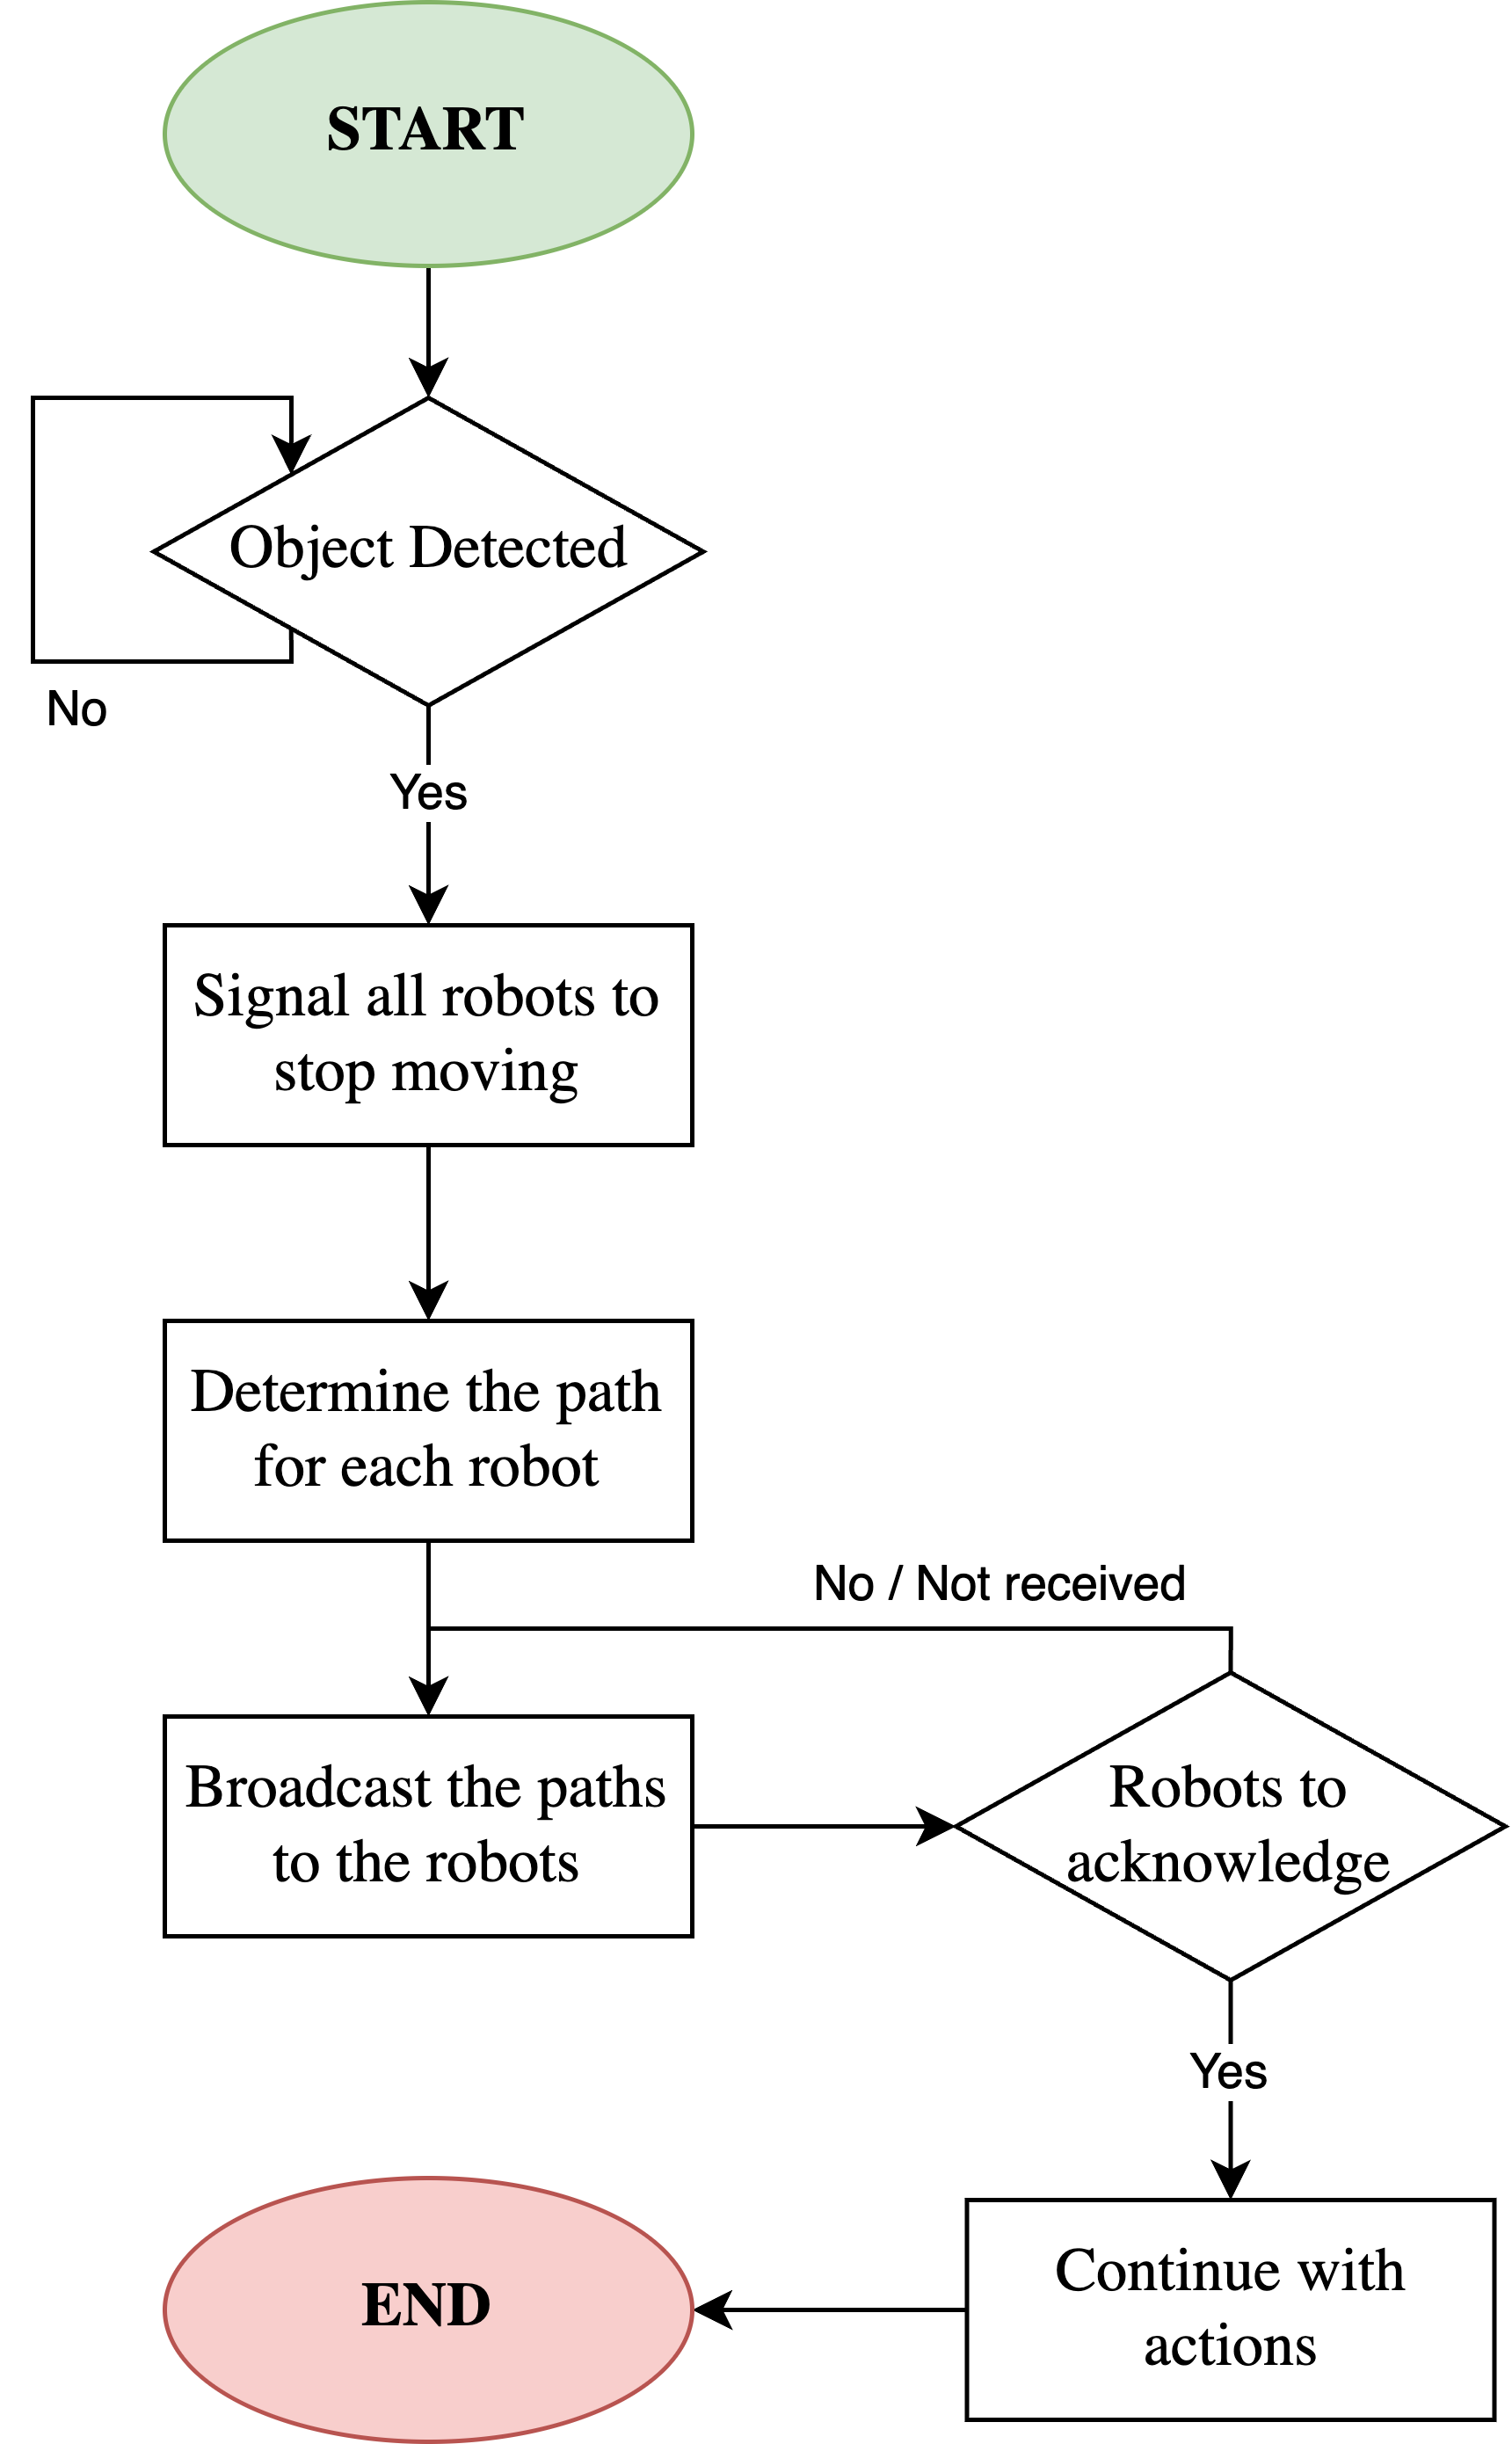
\includegraphics[width=0.5\linewidth]{assets/images/communication/communication-diagram.png}
    \caption{High-level Overview of the Communication Algorithm}
    \label{fig:communication-diagram}
\end{figure}
